\section{The Finite State Machine}
The FSM is the crux of interacting with the CAPP and making it carry out complex arbitrary algorithms by exposing commands to carry out different tasks. 
It has numerous states, some of them are sending or receiving data, loading data into the CAPP, selecting first, searching, reading, setting the comparand and mask as well as writing. 
The base UART module used is from David Things' Github repository. \cite{uart} This works on a 48MHz clock cycle.
To reduce complexities and avoid additional LUTs usage, we used the same clock speed throughout the project. 

\begin{figure}
  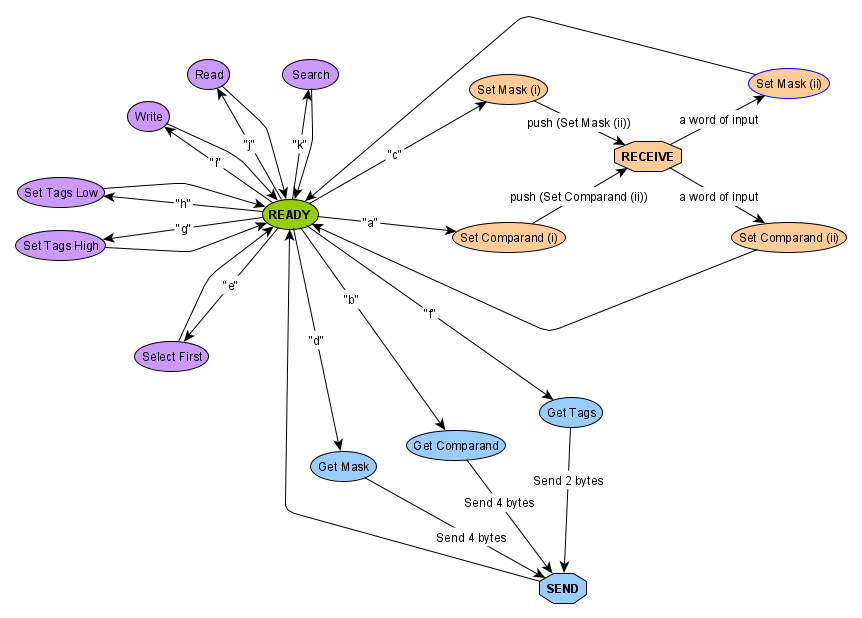
\includegraphics[height=6cm]{FPGA-CAPP research paper/images/protocol.png}
  \caption{Overview of the FSM underlying the CAPP-host protocol}
  \label{FSM_protocol}
\end{figure}

As shown in Figure \ref{FSM_protocol}, our FSM acts as a way to carry out procedural tasks while staying under the limit of 21ns by linking states together. 
Therefore, a task may trigger several states before it returns to the default state. 
For example, the algorithm for searching has several steps, it comprises of
\begin{itemize}
    \item Setting the comparand 
    \item Setting the mask 
    \item Sending the SET signal
    \item Sending the SEARCH signal 
\end{itemize}

Notice that the first two steps use several clock cycles as only one byte of data flows through the UART each clock cycle. 
This is due to its pipeline design. 

The states transitions for the SET signal is given below:
\begin{itemize}
    \item  SET 1: change SET to high, set delay to 5 clock cycles
    \item  IDLE: wait for delay, go to SET 0
    \item  SET 0: change SET to low, listen for new command
\end{itemize}
\vspace{5mm}
This is similar to the SEARCH signal:
\begin{itemize}
    \item  SEARCH 1: change SEARCH to high, set delay to 5 clock cycles
    \item  IDLE: wait for delay, go to SEARCH 0
    \item  SEARCH 0: change SEARCH to low, listen for new command
\end{itemize}
\vspace{5mm}
The tasks that involve transmitting follow a similar state transition procedure. 
Here, a state send one character to the host through the uart each clock cycle. 
Examples of these are sending comparand, tags and mask. 
The state transition diagram for sending the comparand is shown in \ref{FSM_protocol}.
The procedures for the other commands are similar in the way that different states just change the value of a register. 
The send state just transmits data from this register. 
This design decision was made to reduce the memory as well as number of combinatorial circuits. 

\begin{itemize}
    \item  GET COMPARAND: set output text to comparand
    \item  SEND: Send the next character until EOL. Listen for next command
\end{itemize}
